

\documentclass[journal,transmag]{IEEEtran}
\hyphenation{op-tical net-works semi-conduc-tor}

\usepackage{enumitem}

% *** GRAPHICS RELATED PACKAGES ***
%
\ifCLASSINFOpdf
   \usepackage[pdftex]{graphicx}
  % declare the path(s) where your graphic files are
  % \graphicspath{{../pdf/}{../jpeg/}}
  % and their extensions so you won't have to specify these with
  % every instance of \includegraphics
  % \DeclareGraphicsExtensions{.pdf,.jpeg,.png}
\else
  % or other class option (dvipsone, dvipdf, if not using dvips). graphicx
  % will default to the driver specified in the system graphics.cfg if no
  % driver is specified.
  % \usepackage[dvips]{graphicx}
  % declare the path(s) where your graphic files are
  % \graphicspath{{../eps/}}
  % and their extensions so you won't have to specify these with
  % every instance of \includegraphics
  % \DeclareGraphicsExtensions{.eps}
\fi
% graphicx was written by David Carlisle and Sebastian Rahtz. It is
% required if you want graphics, photos, etc. graphicx.sty is already
% installed on most LaTeX systems. The latest version and documentation
% can be obtained at: 
% http://www.ctan.org/pkg/graphicx
% Another good source of documentation is "Using Imported Graphics in
% LaTeX2e" by Keith Reckdahl which can be found at:
% http://www.ctan.org/pkg/epslatex
%
% latex, and pdflatex in dvi mode, support graphics in encapsulated
% postscript (.eps) format. pdflatex in pdf mode supports graphics
% in .pdf, .jpeg, .png and .mps (metapost) formats. Users should ensure
% that all non-photo figures use a vector format (.eps, .pdf, .mps) and
% not a bitmapped formats (.jpeg, .png). The IEEE frowns on bitmapped formats
% which can result in "jaggedy"/blurry rendering of lines and letters as
% well as large increases in file sizes.
%
% You can find documentation about the pdfTeX application at:
% http://www.tug.org/applications/pdftex





\begin{document}

\title{\textsc{Capacidades Caloríficas}}

\author{
\IEEEauthorblockN{David S. Castro , William A. Gómez,  Ana M. Niño, Laura V. Pachón , Juliana Ramos y Luis A. Cañón,}
\IEEEauthorblockA{Pontificia Universidad Javeriana, Bogotá, Colombia}
\IEEEauthorblockA{Informe de laboratorio de Capacidades Caloríficas}
\IEEEauthorblockA{Grupo I}

}
% The paper headers
\markboth{Capacidades Caloríficas. Octubre 13~2021}%
{Shell \MakeLowercase{\textit{et al.}}: Bare Demo of IEEEtran.cls for IEEE Transactions on Magnetics Journals}
\IEEEtitleabstractindextext{%

	\begin{abstract}
	Within this laboratory we will work with calorimetry, which is a process that consists of measuring the heat generated by subjecting a substance to a chemical reaction or change of state.
This laboratory does not need many steps, because with the help of a calorimeter (a measuring instrument that is responsible for recording the amounts of heat supplied or received by the body under study), and knowing what the heat capacity is, you can measure the capacity t the specific heats of different materials, where the first thing that is done is to place a known amount of water at a certain temperature and then pour another material with a much higher temperature, where thanks to the walls of the calorimeter we can assume that the heat given by the substance with higher temperature is equal to the heat received by the substance with lower temperature and the calorimeter.
	\end{abstract}
	\begin{IEEEkeywords}
	 Calorimetry, thermal equilibrium, heat capacity, heat transfer, thermodynamic system, phase change. 
	 	\end{IEEEkeywords}}


\maketitle
\IEEEdisplaynontitleabstractindextext
\IEEEpeerreviewmaketitle


\section{Resumen}

Dentro de este laboratorio trabajaremos el tema de calorimetría, el cual es un proceso que consiste en medir el calor que se genera al someter una sustancia a una reacción química o cambio de estado.
Para este laboratorio no se necesitan muchos pasos, pues con ayuda de un calorímetro (instrumento de medición que se encarga de registrar las cantidades de calor suministradas o recibidas por el cuerpo en estudio), y sabiendo cual es la capacidad calorífica, se puede medir la capacidad y los calores específicos de distintos materiales, donde lo primero que se hace es colocar una cantidad conocida de agua a una temperatura determinada y luego se vierte otro material con una temperatura mucho más alta, donde gracias a las paredes del calorímetro podemos suponer que el calor que da la sustancia con mayor temperatura es igual al calor que recibe la sustancia con menor temperatura y el calorímetro.

\section{Introduction}
	
	El calor (representado con la letra Q) es la energía transferida de un sistema a otro (o de un sistema a sus alrededores) debido en general a una diferencia de temperatura entre ellos. El calor que absorbe o cede un sistema termodinámico depende normalmente del tipo de transformación que ha experimentado dicho sistema.
El principio cero de la termodinámica es cuando dos o más cuerpos en contacto que se encuentran a distinta temperatura alcanzan, pasado un tiempo, el equilibrio térmico (misma temperatura).

El calor específico (o capacidad calorífica específica) es la energía necesaria para elevar en un 1 grado la temperatura de 1 kg de masa. Sus unidades en el Sistema Internacional son J/kg K. Este calor específico multiplicado por la masa y por el cambio de temperatura, corresponde a la energía para que la sustancia cambie dado rango de temperatura, como se muestra a continuación:
 \begin{figure}[!h]
			\center
			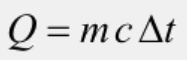
\includegraphics[width=3cm]{img/eq1.png}
			\caption{Calor o Energía de un sistema termodinámico}
			\label{f1}
		\end{figure}

La anterior expresión relaciona la cantidad de calor que intercambia una masa m de una cierta sustancia con la variación de temperatura $\Delta$t que experimenta.  

\begin{figure}[!h]
			\center
			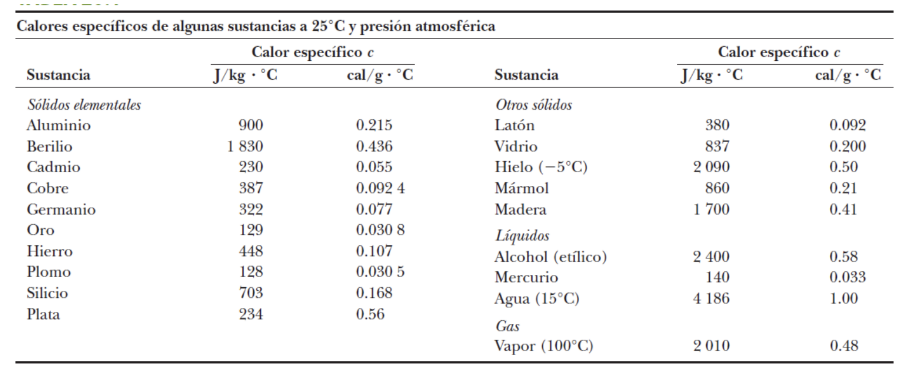
\includegraphics[width=10cm]{img/fig1.png}
			\caption{Calor especifico de algunas sustancias a 25°C.}
			\label{f1}
		\end{figure}

Cuando se produce un \textbf{cambio de fase}, la sustancia debe absorber o ceder una cierta cantidad de calor para que tenga lugar. Este calor será positivo (absorbido) cuando el cambio de fase se produce de izquierda a derecha en la figura, y negativo (cedido) cuando la transición de fase tiene lugar de derecha a izquierda. 
\begin{figure}[!h]
			\center
			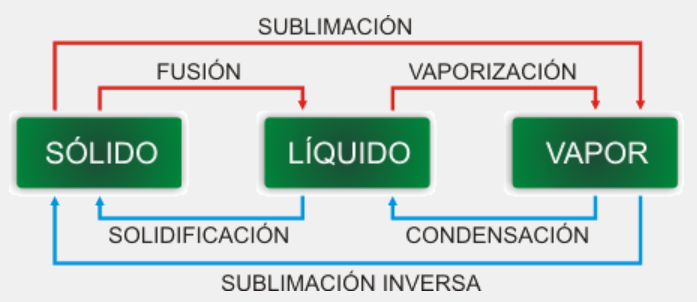
\includegraphics[width=8cm]{img/fig2.png}
			\caption{Cambio de fases entre diferentes estados. }
			\label{f1}
		\end{figure}
		
El calor absorbido o cedido en un cambio de fase no se traduce en un cambio de temperatura, ya que la energía suministrada o extraída de la sustancia se emplea en cambiar el estado de agregación de la materia. Este calor se denomina \textbf{calor latente} . Y se llama así porque, al no cambiar la temperatura durante el cambio de estado, a pesar de añadir calor, éste se quedaba escondido sin traducirse en un cambio de temperatura.

Calor latente (L) o calor de cambio de estado, es la energía absorbida o cedida por unidad de masa de sustancia al cambiar de estado. De sólido a líquido este calor se denomina \textbf{calor latente de fusión}, de líquido a vapor \textbf{calor latente de vaporización} y de sólido a vapor \textbf{calor latente de sublimación}.
El calor latente para los procesos inversos (representados en azul en la figura anterior) tienen el mismo valor en valor absoluto, pero serán negativos porque en este caso se trata de un calor cedido.
En el Sistema Internacional, el calor latente se mide en J/kg.
La cantidad de calor que absorbe o cede una cantidad m de sustancia para cambiar de fase viene dada por:
\begin{figure}[!h]
			\center
			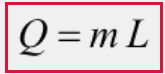
\includegraphics[width=3cm]{img/eq2.png}
			\caption{Energía durante un cambio de fase }
			\label{f1}
		\end{figure}
		
Este calor será positivo o negativo dependiendo del cambio de fase que haya tenido lugar.
%%%%%%%%%%%%%%%%%%%%%%%%%%OBJETIVOS
\section{Objetivos}

	\begin{enumerate}
		\item Entender la noción de calor.
		\item Utilizar el primer principio de la termodinámica.
		\item Diferenciar entre variables de estado y variables de proceso.
		\item Poder calcular capacidades caloríficas y calores específicos de diferentes sistemas. 
	\end{enumerate}
	

%%%%%%%%%%%%%%%%%%%%%%%%%%METODOLOGIA
\section{Metodología}

El laboratorio fue realizado con los materiales que se enumeran a continuación:
	\begin{enumerate}
	
  \item Agua y vaso de precipitado:
		\begin{figure}[!h]
			\center
			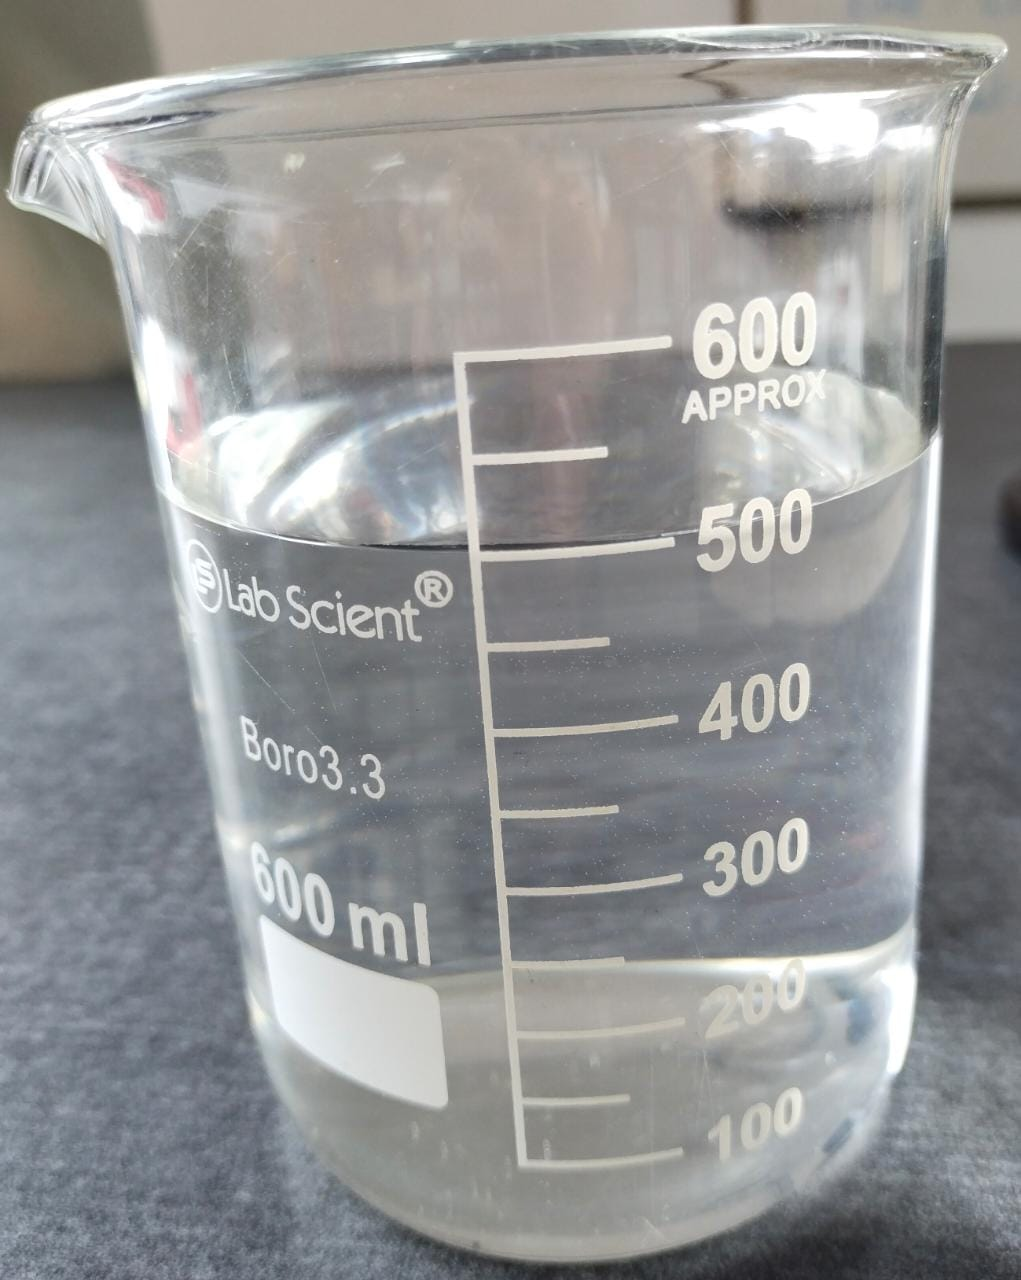
\includegraphics[width=3cm]{img/agua.jpeg}
			\caption{Agua a temperatura ambiente}
			\label{f1}
		\end{figure}
		
	Agua de la llave que se dejó reposar durante varios minutos después de sacada del grifo. Se midió su temperatura inicial y registro 20°C. El vaso de precipitado se encuentra a esta misma temperatura. Finalmente se utilizó 200 mL de agua debido a la capacidad del calorímetro.
		\vspace{20mm}
  \item Calorímetro:
  \begin{figure}[!h]
			\center
			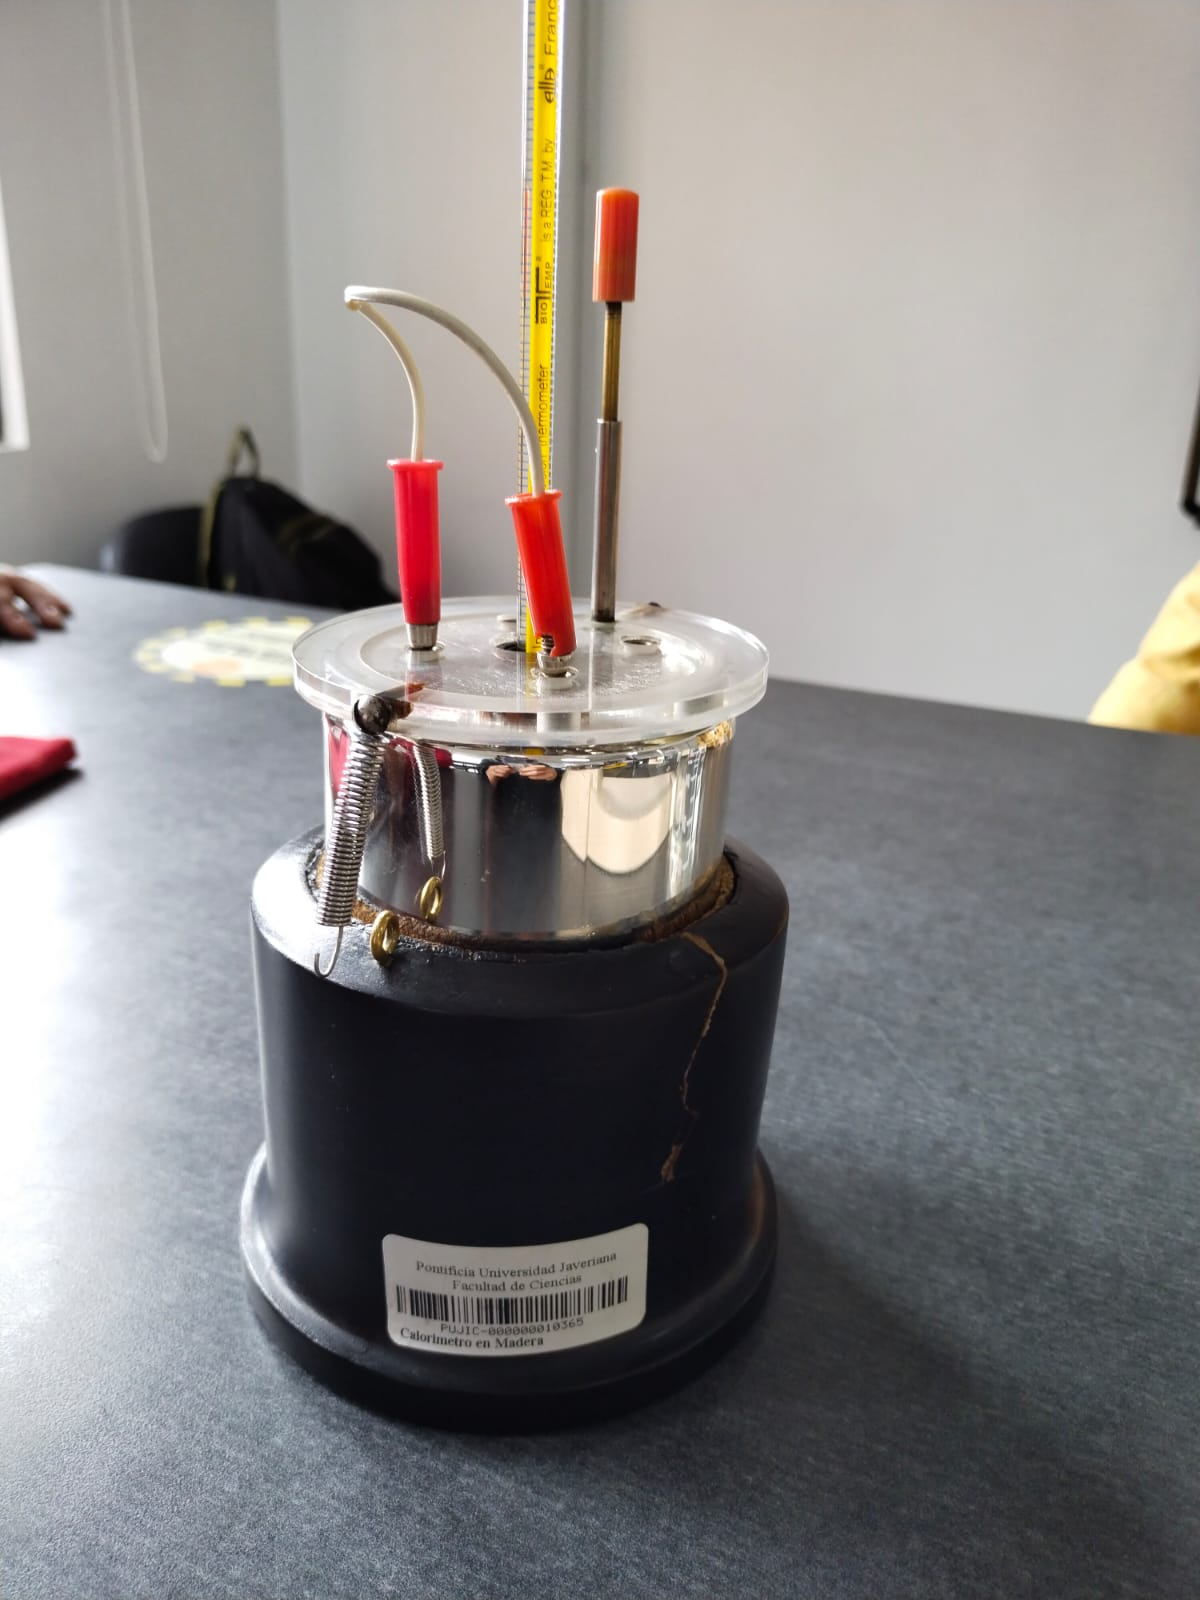
\includegraphics[width=3cm]{img/calorimetro.jpeg}
			\caption{Calorímetro}
			\label{f3}
		\end{figure}
		
	Un calorímetro del laboratorio de Física de la universidad; esta compuesto con un interior reflector y un exterior de madera para asegurar la menor transferencia de energía entre las paredes del calorímetro y el ambiente. 

  \item Termómetro: 
  \begin{figure}[!h]
			\center
			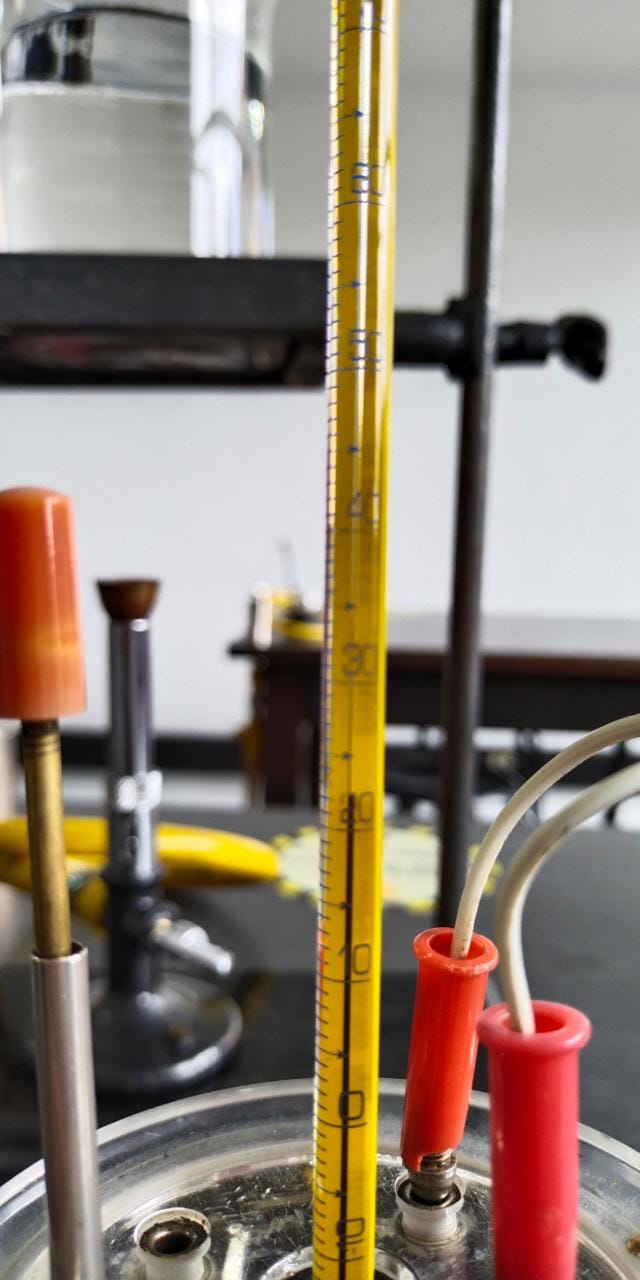
\includegraphics[width=3cm]{img/termometro.jpeg}
			\caption{Termómetro de mercurio .}
			\label{f2}
		\end{figure}
		
	Con este termómetro de mercurio registramos la temperatura inicial del agua, también la temperatura final de esta; ademas fue utilizado para medir los cambios de temperatura con respecto al tiempo que ocurrieron en el segundo Experimento.

 \item Balanza de tres brazos
			\begin{figure}[!h]
				\center
				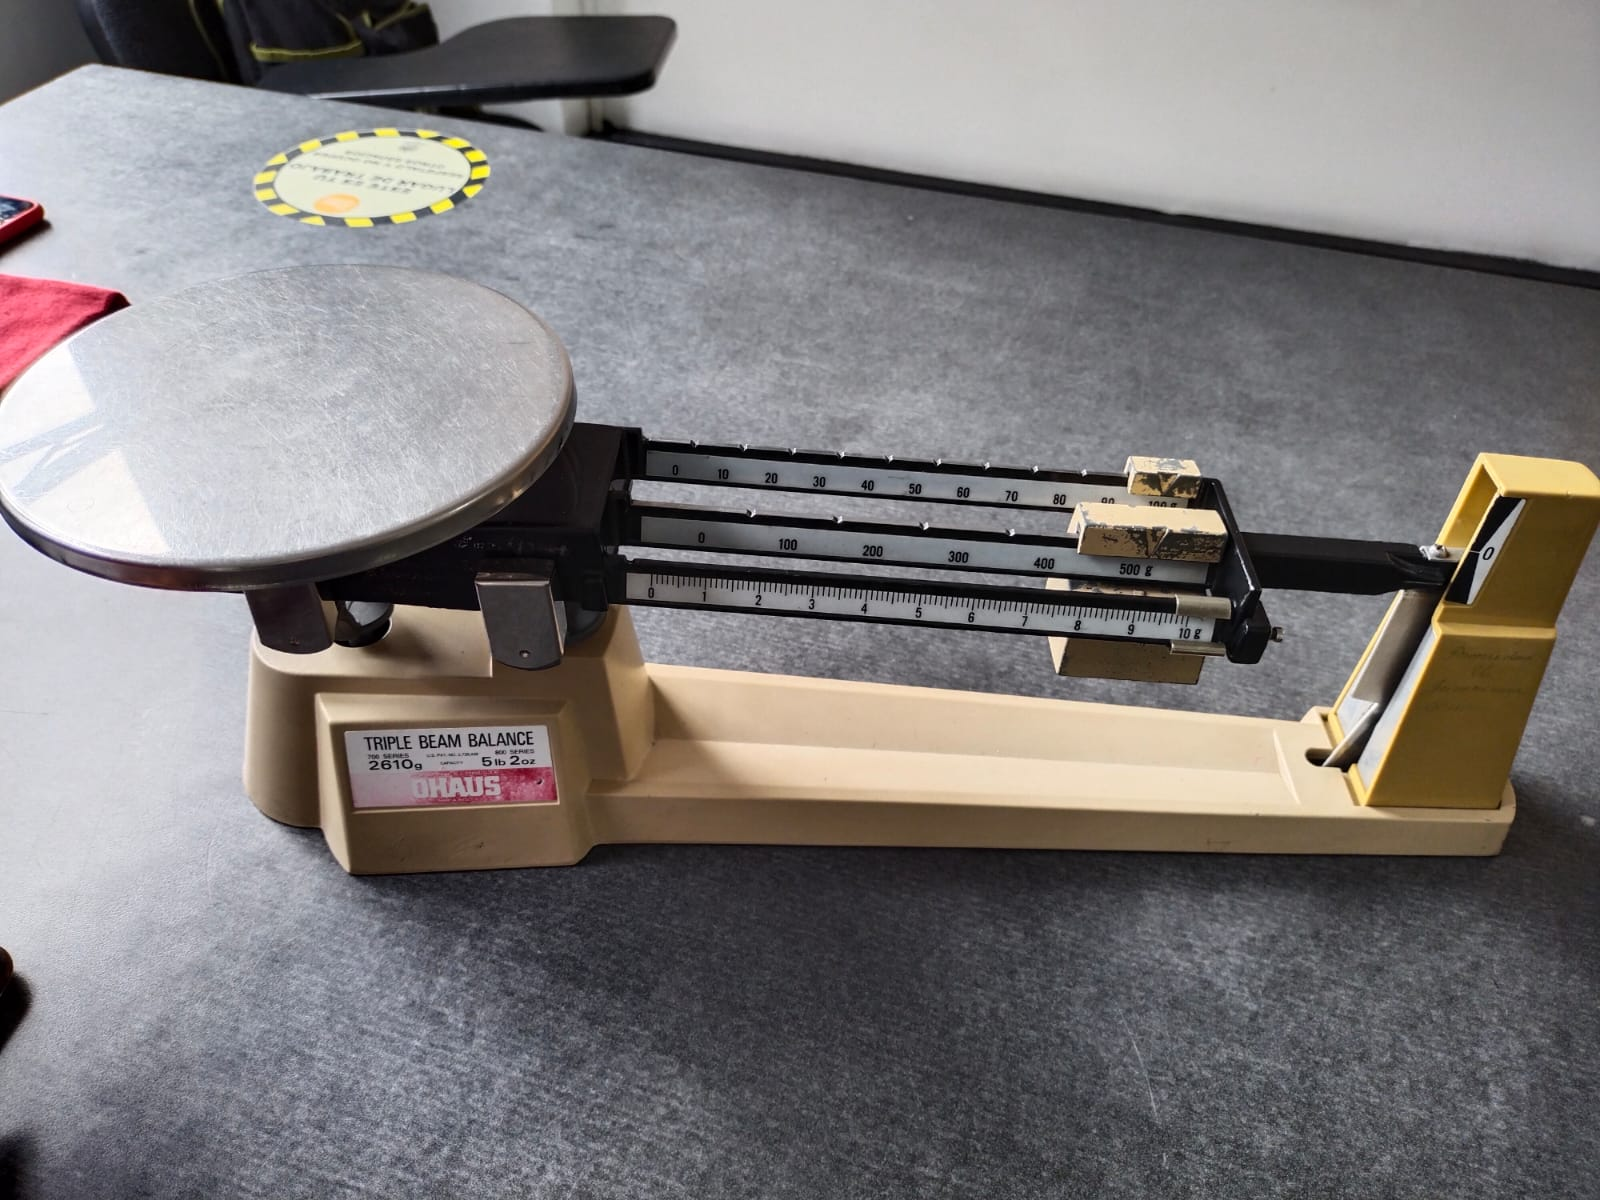
\includegraphics[width=6cm]{img/pesa.jpeg}
				\caption{Balanza}
				\label{f4}
			\end{figure}
			
	Esta balanza fue utilizada para medir la masa del calorímetro del vidrio, ademas medimos la masa inicial y final del agua (antes de llevarla a su temperatura de ebullición y después).

\item Mechero
			\begin{figure}[!h]
				\center
				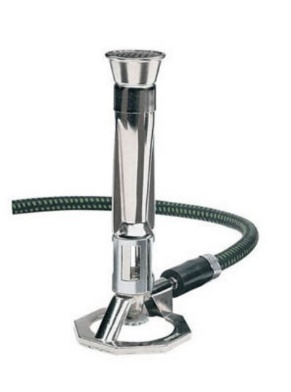
\includegraphics[width=3cm]{img/mechero.jpg}
				\caption{Mechero}
				\label{f4}
			\end{figure}
	\end{enumerate}

Este mechero fue utilizado junto con la estructura metálica de la Figura \ref{fi1} para realizar el Experimento 1 y otorgar energía a el sistema vidrio + agua.

\vspace{5mm}

 Estos elementos fueron utilizados para hacer 2 experimentos distintos; en primer lugar calculamos la energía o calor necesario para hacer ebullir 200 mL de agua a temperatura ambiente (20°C). Para esto fue necesario contar con el montaje de la figura \ref{fi1}, en donde ubicamos el vaso de precipitado de vidrio con el agua sobre una plancha que calentamos con ayuda de un mechero. 
 \begin{figure}[!h]
				\center
				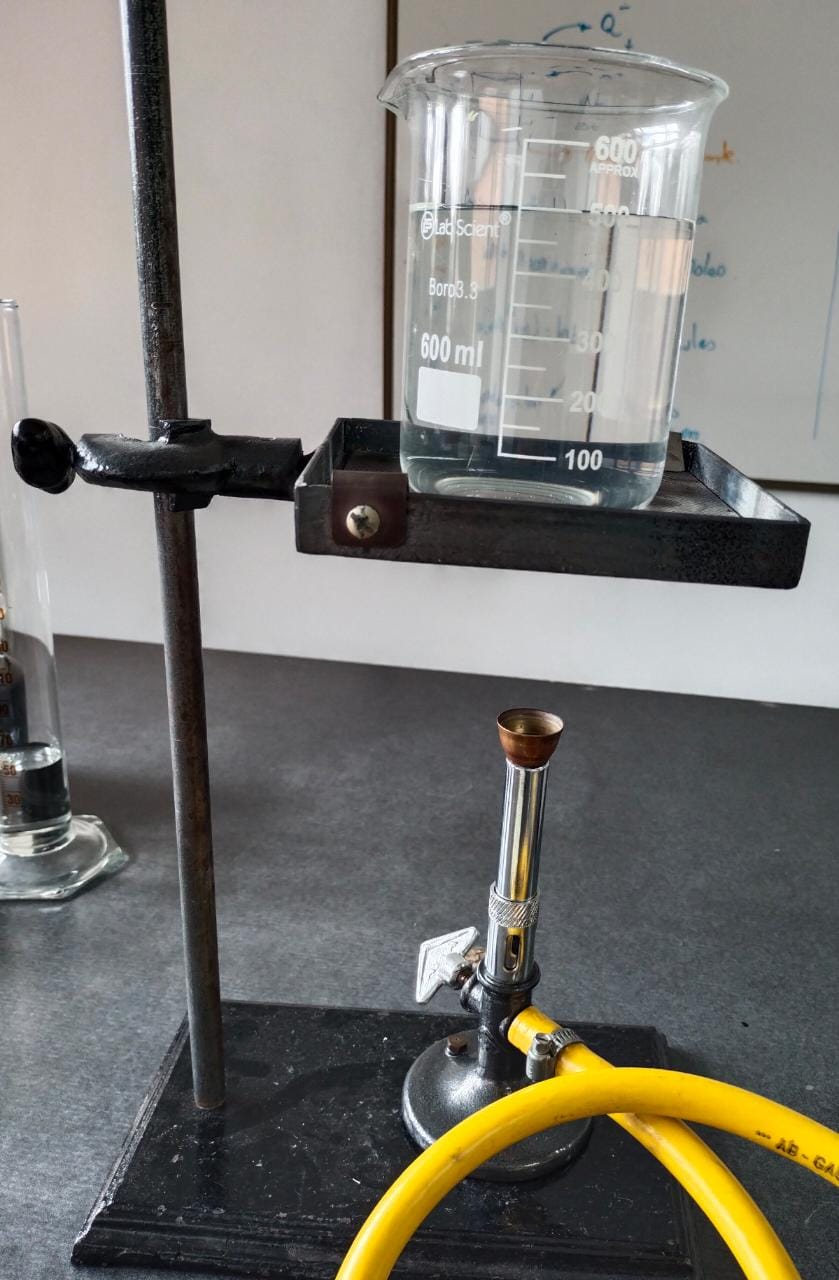
\includegraphics[width=6cm]{img/montaje.jpeg}
				\caption{Montaje utilizado para subir la temperatura del agua liquida hasta su máximo (Punto de ebullición)}
				\label{fi1}
			\end{figure}
 

 Por otro lado, una vez el agua liquida estaba a su máxima temperatura posible (87°C), la vertimos en el calorímetro y observamos la temperatura hasta que se llegara a un equilibrio de temperatura por un tiempo constante. Con esta temperatura de equilibrio procedimos a calcular la capacidad calorífica del calorímetro. 

Es decir, vamos a determinar un volumen especifico de agua que se va a colocar en el vaso precipitado y vamos a pesarlo con la balanza de tres brazos, para posteriormente calentarlo con la ayuda del termómetro de mercurio y del mechero hasta una temperatura de alrededor del 92 °C (temperatura de ebullición en Bogotá) o lo mas caliente posible sin que se evapore mucho el agua. Luego, se coloca el agua que se calentó en el vaso precipitado en el calorímetro y se sigue tomando la temperatura para saber cual es su temperatura de equilibrio.
Para saber cual era la temperatura de equilibrio entre el calorímetro y el agua simplemente debíamos ver cuando la temperatura comenzaba a descender a una menor velocidad y ahí podíamos inferir que habían llegado a un equilibrio térmico. Con la explicación anterior, ya se acabó la parte práctica y de recolección de datos del laboratorio, ahora teníamos que calcular cual era el calor añadido a el agua y cual era el calor especifico del calorímetro.



%%%%%%%%%%%%%%%%%%%%%%%%%%RESULTADOS
\section{Resultados} 

\subsection{Experimento 1: Energía necesaria para ebullir 200 mL de agua}

Para el primer experimento, nuestra intención era simplemente subir la temperatura del agua hasta su punto de ebullición; según nuestra presión atmosférica de Bogotá se determino que esta temperatura era de 92°C, sin embargo esta temperatura no logró alcansarce y el agua empezó a evaporarse a los 87° C. En este proceso se perdió una cantidad significativa de agua, por esto, se decidió tomar dos valores para la masa del agua. La masa del agua inicial fue 352.5 gramos, mientras que la masa final de este experimento fue 323.5.

A continuación se muestran los cálculos realizados y la respuesta obtenida para el Experimento 1.

\begin{figure}[!h] 
	\center 
	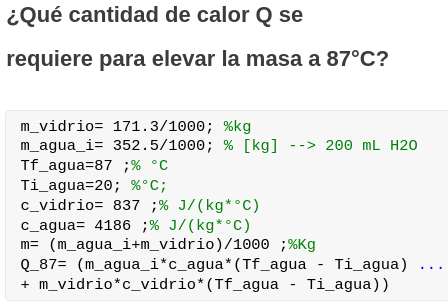
\includegraphics[width=8cm]{img/ans1.png} 
	\caption{Cálculos hechos en Matlab para hallar la energía suministrada al sistema} 
	\label{T4} 
\end{figure} 
\begin{figure}[!h] 
	\center 
	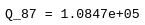
\includegraphics[width=5cm]{img/ans11.png} 
	\caption{Resultado del Calor o Energía necesaria para elevar la temperatura del agua y del vaso de vidrio desde 20°C hasta 87°C. Unidades [J]} 
	\label{T4} 
\end{figure} 

Se puede observar entonces que la energía requerida para subir la temperatura del sistema hasta el punto de ebullición del agua es de  $ 1.08e10^5$ Joules.
Para este cálculo se tuvo en cuenta que no existió ningún cambio de fase de ningún elemento ni agua ni vidrio. Por lo tanto la energía requerida sera la suma de la energía requerida para llevar cada componente a dicha temperatura final.


\subsection{Experimento 2: Hallar el calor específico del Calorímetro}

Una vez el agua estaba hirviendo la agregamos directamente en el calorímetro frio ( a temperatura ambiente 20°C) e insertamos el termómetro para observar el cambio de la temperatura. Una vez transcurrido un tiempo y haber hecho diferentes observaciones entre todo el grupo, se determino que la temperatura de equilibrio que tomaríamos como la temperatura final del sistema agua + calorímetro era de 68°C.
Estas observaciones se pueden ver en la siguiente gráfica:

\begin{figure}[!h] 
	\center 
	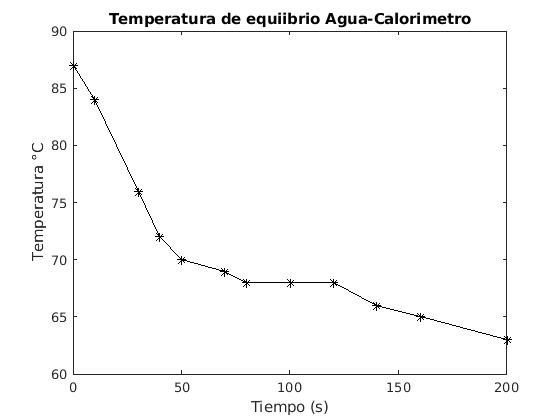
\includegraphics[width=7cm]{img/grafica.jpg} 
	\caption{Grafica: Temperatura del sistema agua caliente + calorímetro, en función del tiempo. Se quiere determinar la temperatura de equilibrio.} 
	\label{T4} 
\end{figure} 


Ya que la energía no se crea ni se destruye, solo se transforma, la energía cedida en el sistema más la energía ganada sera igual a cero. Por lo tanto calculamos la capacidad calorífica del calorímetro plantando esta ecuación.
Estos cálculos se muestran a continuación:

\begin{figure}[!h] 
	\center 
	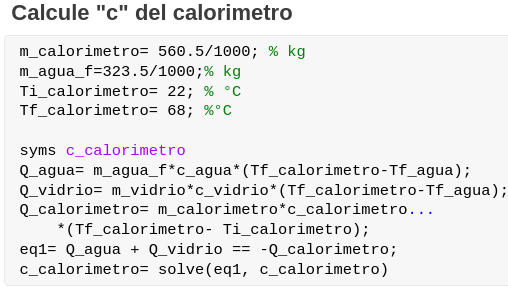
\includegraphics[width=8cm]{img/ans2.png} 
	\caption{Cálculos hechos en Matlab para hallar el calor específico del calorímetro} 
	\label{T4} 
\end{figure} 
\begin{figure}[!h] 
	\center 
	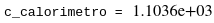
\includegraphics[width=7cm]{img/ans22.png} 
	\caption{Calor especifico del Calorímetro. Unidades [J/kg°C]} 
	\label{T4} 
\end{figure} 

Finalmente obtuvimos que la capacidad calorífica del calorímetro era $ 1.10e10^3$  J/kg°C

%%%%%%%%%%%%%%%%%%%%%%%%%%%%%%%%%%%%%%%%%%%%%%%%%%%%RESULTADOS

\section{Análisis de resultados}
El en el primer experimento fue necesario que la llama de fuego calentara una plancha térmica, la cual se caracteriza por tener un punto de ebullición  y una capacidad calorífica muy altos. Por lo tanto la plancha caliente captura rápidamente la energía que es liberada por la llama de fuego y a su vez la transmite directamente a el vaso de vidrio. Este vaso de vidrio esta en contacto con el agua, por lo que la temperatura del agua será la misma que la temperatura del vidrio. Una vez la temperatura llega a 90°C a aproximadamente dejara de subir la temperatura y comenzara a evaporarse todo el agua. Esto quiere decir que la llama de fuego a pesar de seguir inyectando calor a el sistema, el sistema no cambiara de temperatura, esto debido a que el sistema esta compuesto por un elemento que se encuentra en su temperatura  de cambio de fase, el agua liquida se va a convertir en vapor a esta temperatura (que depende de la presión atmosférica), por l tanto toda esta energía sera utilizada para transformar toda el agua liquida en vapor y mientras tanto el vidrio estará a la misma temperatura del agua hirviendo.

Para el experimento 2 habíamos observado que bastante agua se había evaporado y decidimos medir esta masa de agua para iniciar el experimento 2, el cual consistió en buscar la temperatura de equilibrio del agua hirviendo a 87°C con el calorímetro a temperatura ambiente de 22°C. La temperatura de equilibrio fue 68°C y esto nos permitió hallar la capacidad calorífica del calorímetro. Una vez se enfrió el agua la sacamos del calorímetro y la pesamos.

Al final pudimos determinar que se requirieron $ 1.08e10^5$ Joules para elevar la temperatura de 200 mL de agua desde 20°C hasta 87°C, aproximadamente. Mientras que la capacidad calorífica de el calorímetro del laboratorio de física tiene un valor de $ 1.10e10^3$  J/kg°C.

Vale destacar que una fuente de error considerable surgió cuando medimos la temperatura de equilibrio, ya que los datos registrados de tiempo vs temperatura no se hicieron de manera ordenada y los datos contenían muy pocos datos, tuvimos que reconstruir de la mejor manera la información para decidir entre todo el grupo cual sería la temperatura de equilibrio, introduciendo obviamente algo de error en esta temperatura. Por otro lado, la temperatura del calorímetro fue tomada como la temperatura inicial del agua , pero no estamos seguros que el calorímetro y el agua tuvieran la misma temperatura.


\section{Conclusión}
	
	\begin{enumerate}[label=(\roman*)]
		\item Pudimos determinar con éxito la energía requerida para cambiar la temperatura del sistema termodinámico agua + vidrio a una temperatura de ebullición del agua, partiendo de la temperatura ambiente. 
		\item  Calculamos la capacidad calorífica de un calorímetro utilizando la técnica de ponerlo en contacto con un elemento de temperatura y masa conocidas para determinar la temperatura de equilibrio de este sistema. 
		\item  Sin importar cuanto calor se le trasmita a un sistema durante un cambio de fase, este no elevará su temperatura, utilizara toda la energía para transformar el elemento del sistema de una fase a otra.
		\item Dos cuerpos en contacto, después de un tiempo, tendrán la misma temperatura.
	\end{enumerate}

\appendices


\ifCLASSOPTIONcaptionsoff
  \newpage
\fi


\begin{thebibliography}{1}


 \bibitem{IEEEhowto:Monteria}
 Martin T. y Serrano A. (s.f) calor. Recuperado de: https://www2.montes.upm.es/dptos/digfa/cfisica/termo1p/calor.html

 \bibitem{IEEEhowto:Monteria}
 Mechero: $https://assets.fishersci.com/TFS-Assets/CCG/product-images/15311802_A.JPG-650.jpg $

\end{thebibliography}



\end{document}